\subsection{3D Modell\hfill\textnormal{\emph{Berger}}}

Der grundsätzliche Aufbau des Roboters hat sich nach dem kombinierten Prototypen nicht groß verändert.
Die Aufgabe des finalen Modells war es also eher 
genauer zu definieren aus welchen Bauteilen der Roboter besteht
und zu beweisen das alle angedachten Funktionen im Gerät unterzubringen sind.

Wie in Abbildung \ref{fig:model_open_front} zu sehen, 
besteht der finale Roboter aus einer großen Grundplatte, 
die durch eine Rückwand und einen Deckel abgedeckt wird.
Dies vereinfacht die Wartung der inneren Komponenten
und erlaubt das komplette ausbauen der beiden Container.

\begin{figure}[H]
  \centering{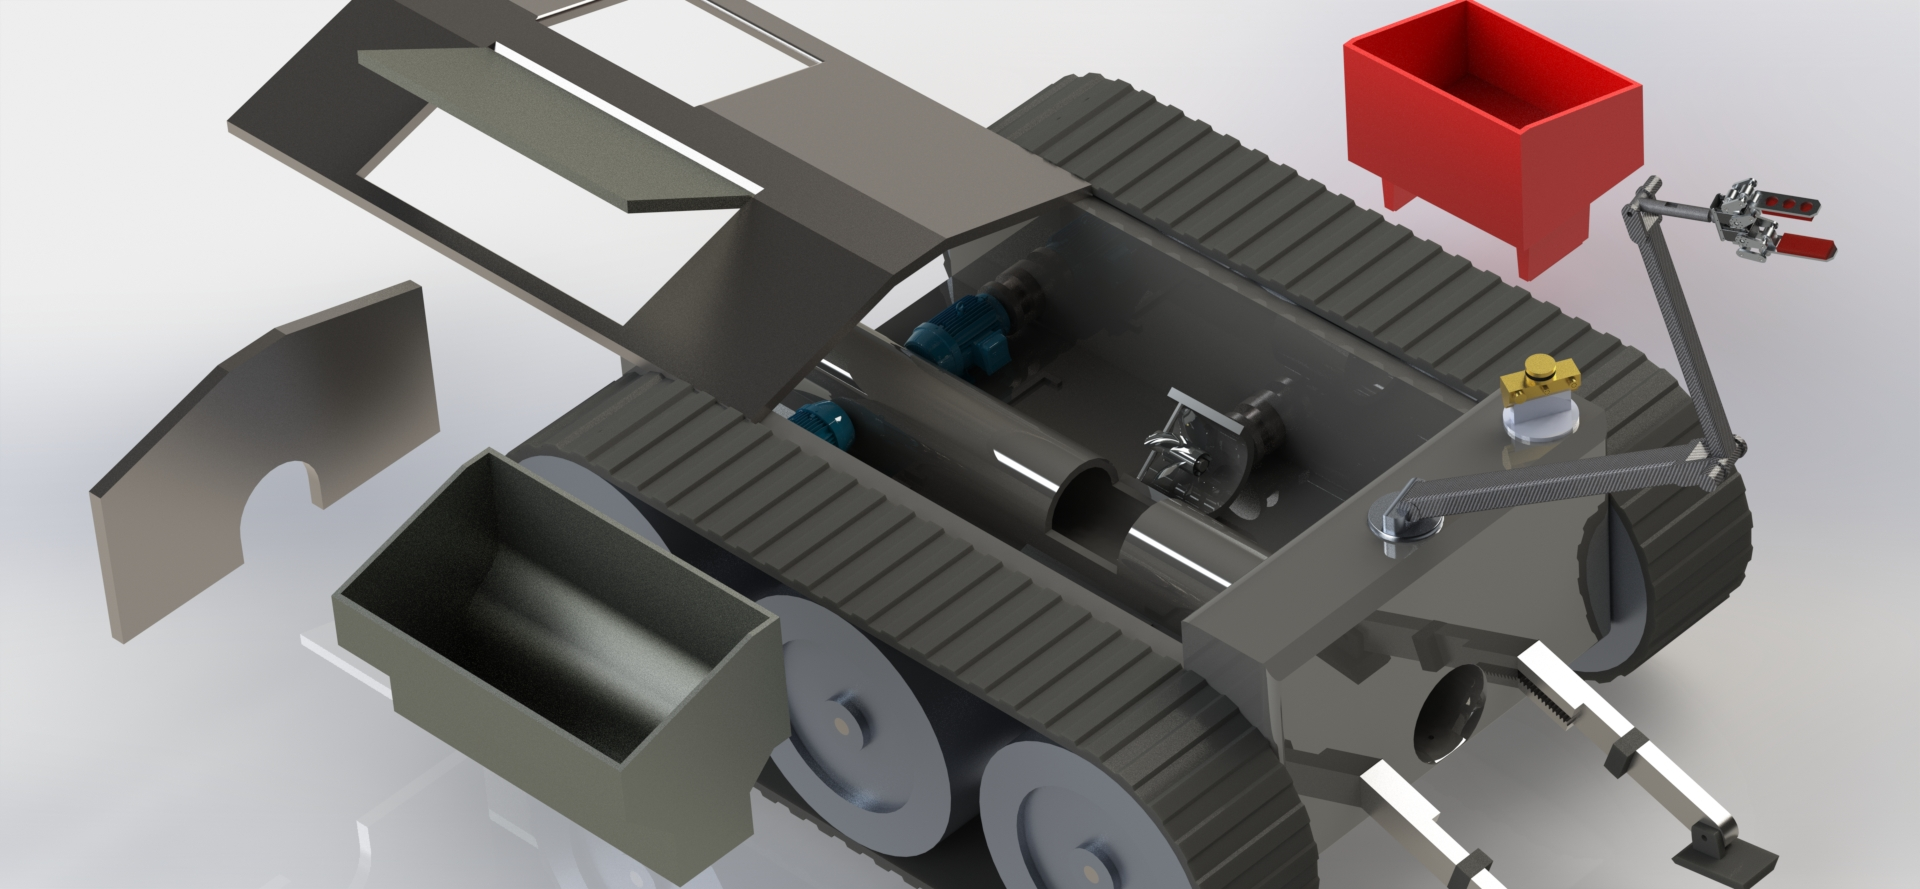
\includegraphics[width=1.0\linewidth]{Abbildungen/3D_model/final_open_front_2.JPG}}
  \caption{Modell final TEST}
  \label{fig:model_open_front}
\end{figure}

Die Ketten wurden um relativ sanfte Zähne erweitert 
um die Griff-Fähigkeit auf losem Untergrund zu verbessern.
Sie werden angetrieben durch jeweils einen Elektromotor,
der am hinteren Rad angebracht ist,
besonders gut zu sehen in Abbildung \ref{fig:model_open_back}.

In der Mitte der Grundplatte befindet sich eine Aussparung in der Wasser-Röhre.
Dort wird der Propeller an einer Klappe befestigt,
die wie in Abbildung \ref{fig:model_open_front} gezeigt
aufgeklappt werden kann, 
zur Installation oder Wartung.

\begin{figure}[H]
  \centering{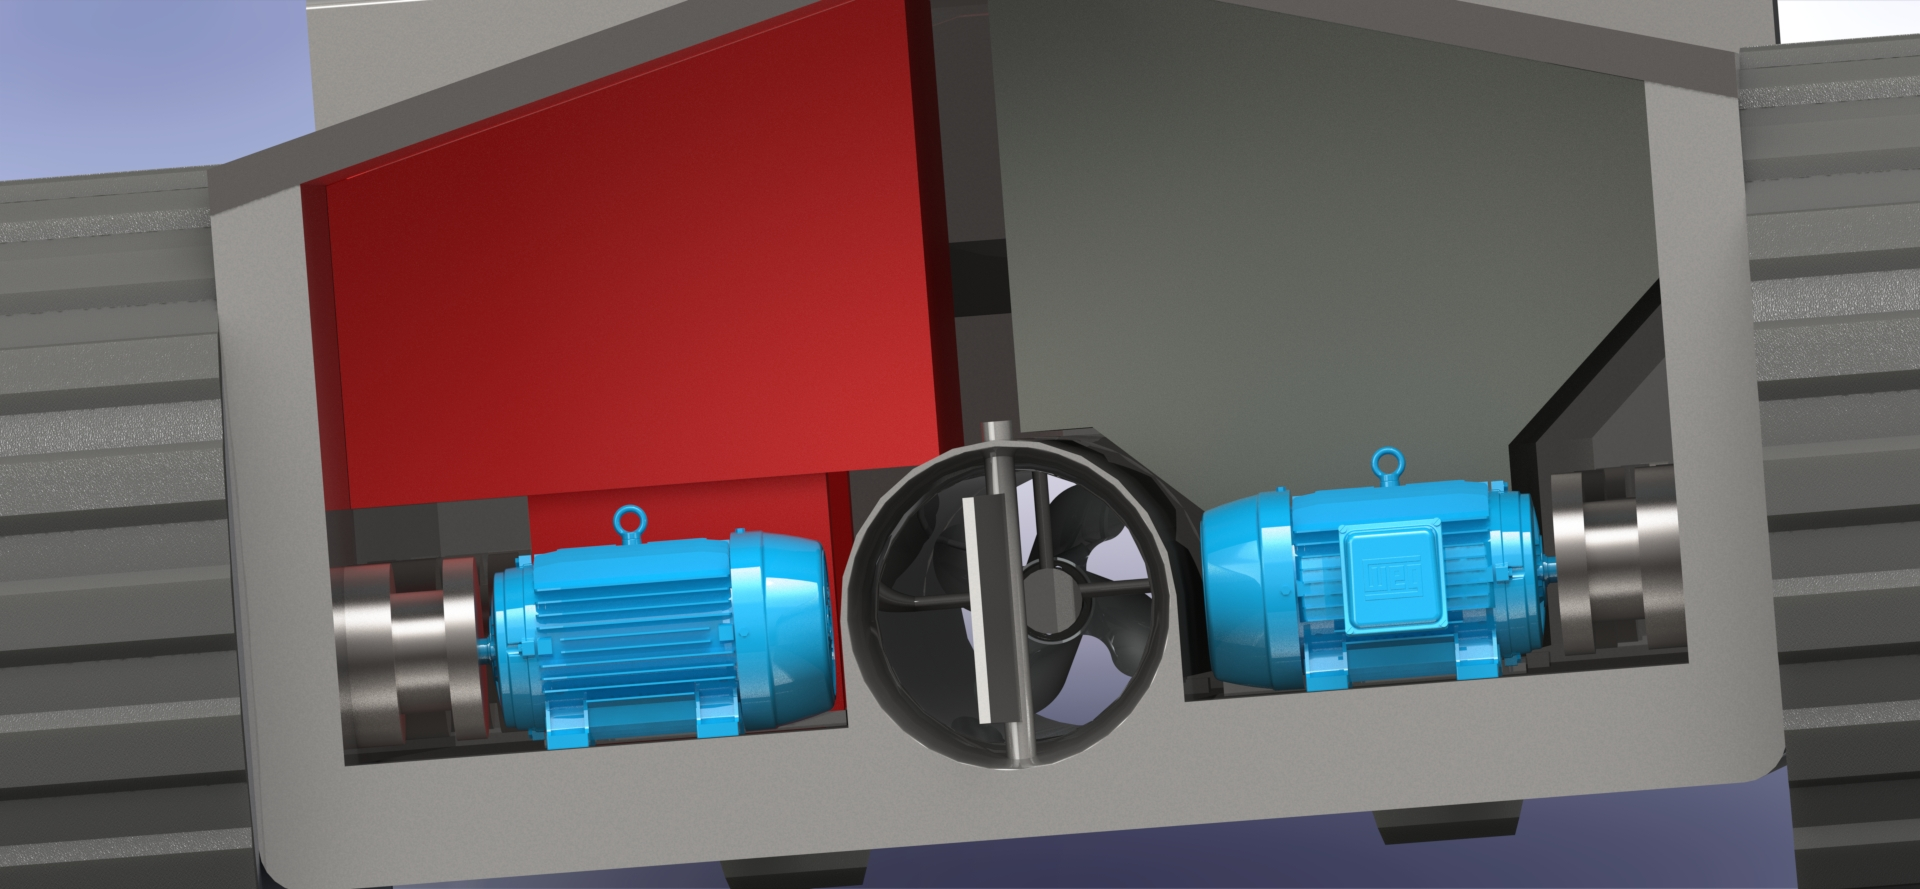
\includegraphics[width=1.0\linewidth]{Abbildungen/3D_model/final_open_back.JPG}}
  \caption{Modell back}
  \label{fig:model_open_back}
\end{figure}